\documentclass[a4paper,14pt]{extarticle}
\usepackage[left=2.5cm, right=1.5cm, vmargin=2.5cm]{geometry}
\usepackage[utf8]{inputenc}
\usepackage[T2A]{fontenc}
\usepackage[russian]{babel}
\usepackage{graphicx}
\graphicspath{{pictures/}}
\usepackage{caption}
\usepackage{subcaption}
\usepackage{indentfirst}
\setlength\parindent{5ex}
\usepackage{fancyhdr}
\usepackage{booktabs}
\usepackage{siunitx} 
\usepackage{pgfplotstable}
\usepackage{amsmath}
\usepackage{autonum}
\usepackage{amsfonts}
\DeclareMathOperator{\sign}{sgn}
\newcommand{\gt}{\textgreater} % знак больше
\newcommand{\lt}{\textless}       % знак меньше
\DeclareGraphicsExtensions{.pdf,.png,.jpg}
\pagestyle{fancy}
\fancyhf{}
\rhead{\thepage}
\renewcommand{\headrulewidth}{0pt}

\fancypagestyle{plain}{ 
	\fancyhf{}
	\rhead{\thepage}}

\author{Никитин Илья}

\title{Отчет по лабораторной работе №1: "Вводная лабораторная работа. Генератор Ван Дер Граафа"}
\date{\today}

\begin{document}
	
	\maketitle
	\tableofcontents
	
	\section{Вводная лабороторная работа}
		\tableofcontents
		\subsection{Оборудование}
			\begin{itemize}
				\item Цифровой осциллограф со встроенным генератором различных
				форм напряжения
				\item Щуп для осциллографа – 3 шт.
				\item Мультиметр
				\item Переменное сопротивление 
				\item Катушки индуктивности 
				\item Диод 
				\item Макетная плата 
				\item Соединительные провода 
				\item Источник постоянного тока 
				\item Щупы для мультиметра 
				\item Латунный образец малого сопротивления
			\end{itemize}
		\subsection{Задачи}
			\begin{itemize}
				\item Определение индуктивности катушки
				\item Снятие ВАХ диода
				\item Измерение малого сопротивления
			\end{itemize}
		\subsection{Определение индуктивности катушки}
			\subsubsection{Теория работы}
				\begin{figure}[h]
					\centering
					\includegraphics[width=.75\linewidth]{схема.png}
					\caption{Схема измерения индуктивности. $R$ – резистор сопротивлением 480 Ом, $L$ – катушка, индуктивность которой требуется измерить (заявлено 1мГн), $G$ – выход встроенного	генератора осциллографа, $U_1$ и $U_2$ – напряжения, измеряемое на первом и втором каналах осциллографа. Земля у генератора и обоих входов осциллографа общая.}
					\label{fig1}
				\end{figure}
				\newpage
				С генератора подается синусоидальный сигнал с амплитудой 12 В. В приближении, что резистор имеет только активное сопротивление, а катушка только реактивное можно рассчитать импеданс катушки $Z_L = i \omega L$ зная $U_1$, $U_2$ и $R$. Полный импеданс всей цепи равен $Z_\Sigma =	R + i \omega L$. Тогда модули (и амплитуды) тока и напряжения в цепи связаны следующим образом: $U_0 = I_0 \sqrt{R^2 + (\omega L)^2}$. Также из этого легко найти модуль тангенса разности фаз между током и напряжением: $tan(\phi) = \frac{\omega L}{R}$. Измеряемое напряжение $U_2$ равно произведению величины тока в цепи на сопротивление $R$, из это получим связь между $U_1$ и $U_2$: $\frac{U_1}{U_2} = \sqrt{1 + (\frac{\omega L}{R})^2}$, из которой можно найти индуктивность $L$. Из этого соотношения легко понять требования на величину сопротивления $R$ и частоту $\omega$: они должны быть такими, чтобы величина $\frac{\omega L}{R}$ заметно превышала единицу, иначе измерения будут неточными.
			\subsubsection{Ход работы}
				В ходе работы с помощью осциллографа на заданной схеме были измерены напряжения на катушке для различных частот, затем определены различные значения выражения $\frac{R}{2\pi}\sqrt{(\frac{U_1}{U_2})^2 - 1}$ при различных значениях частоты, а затем были построене прямые по МНК и взвешенному МНК, коэффициентом которых является искомая индуктивность катушки
				\begin{figure}[h]
					\centering
					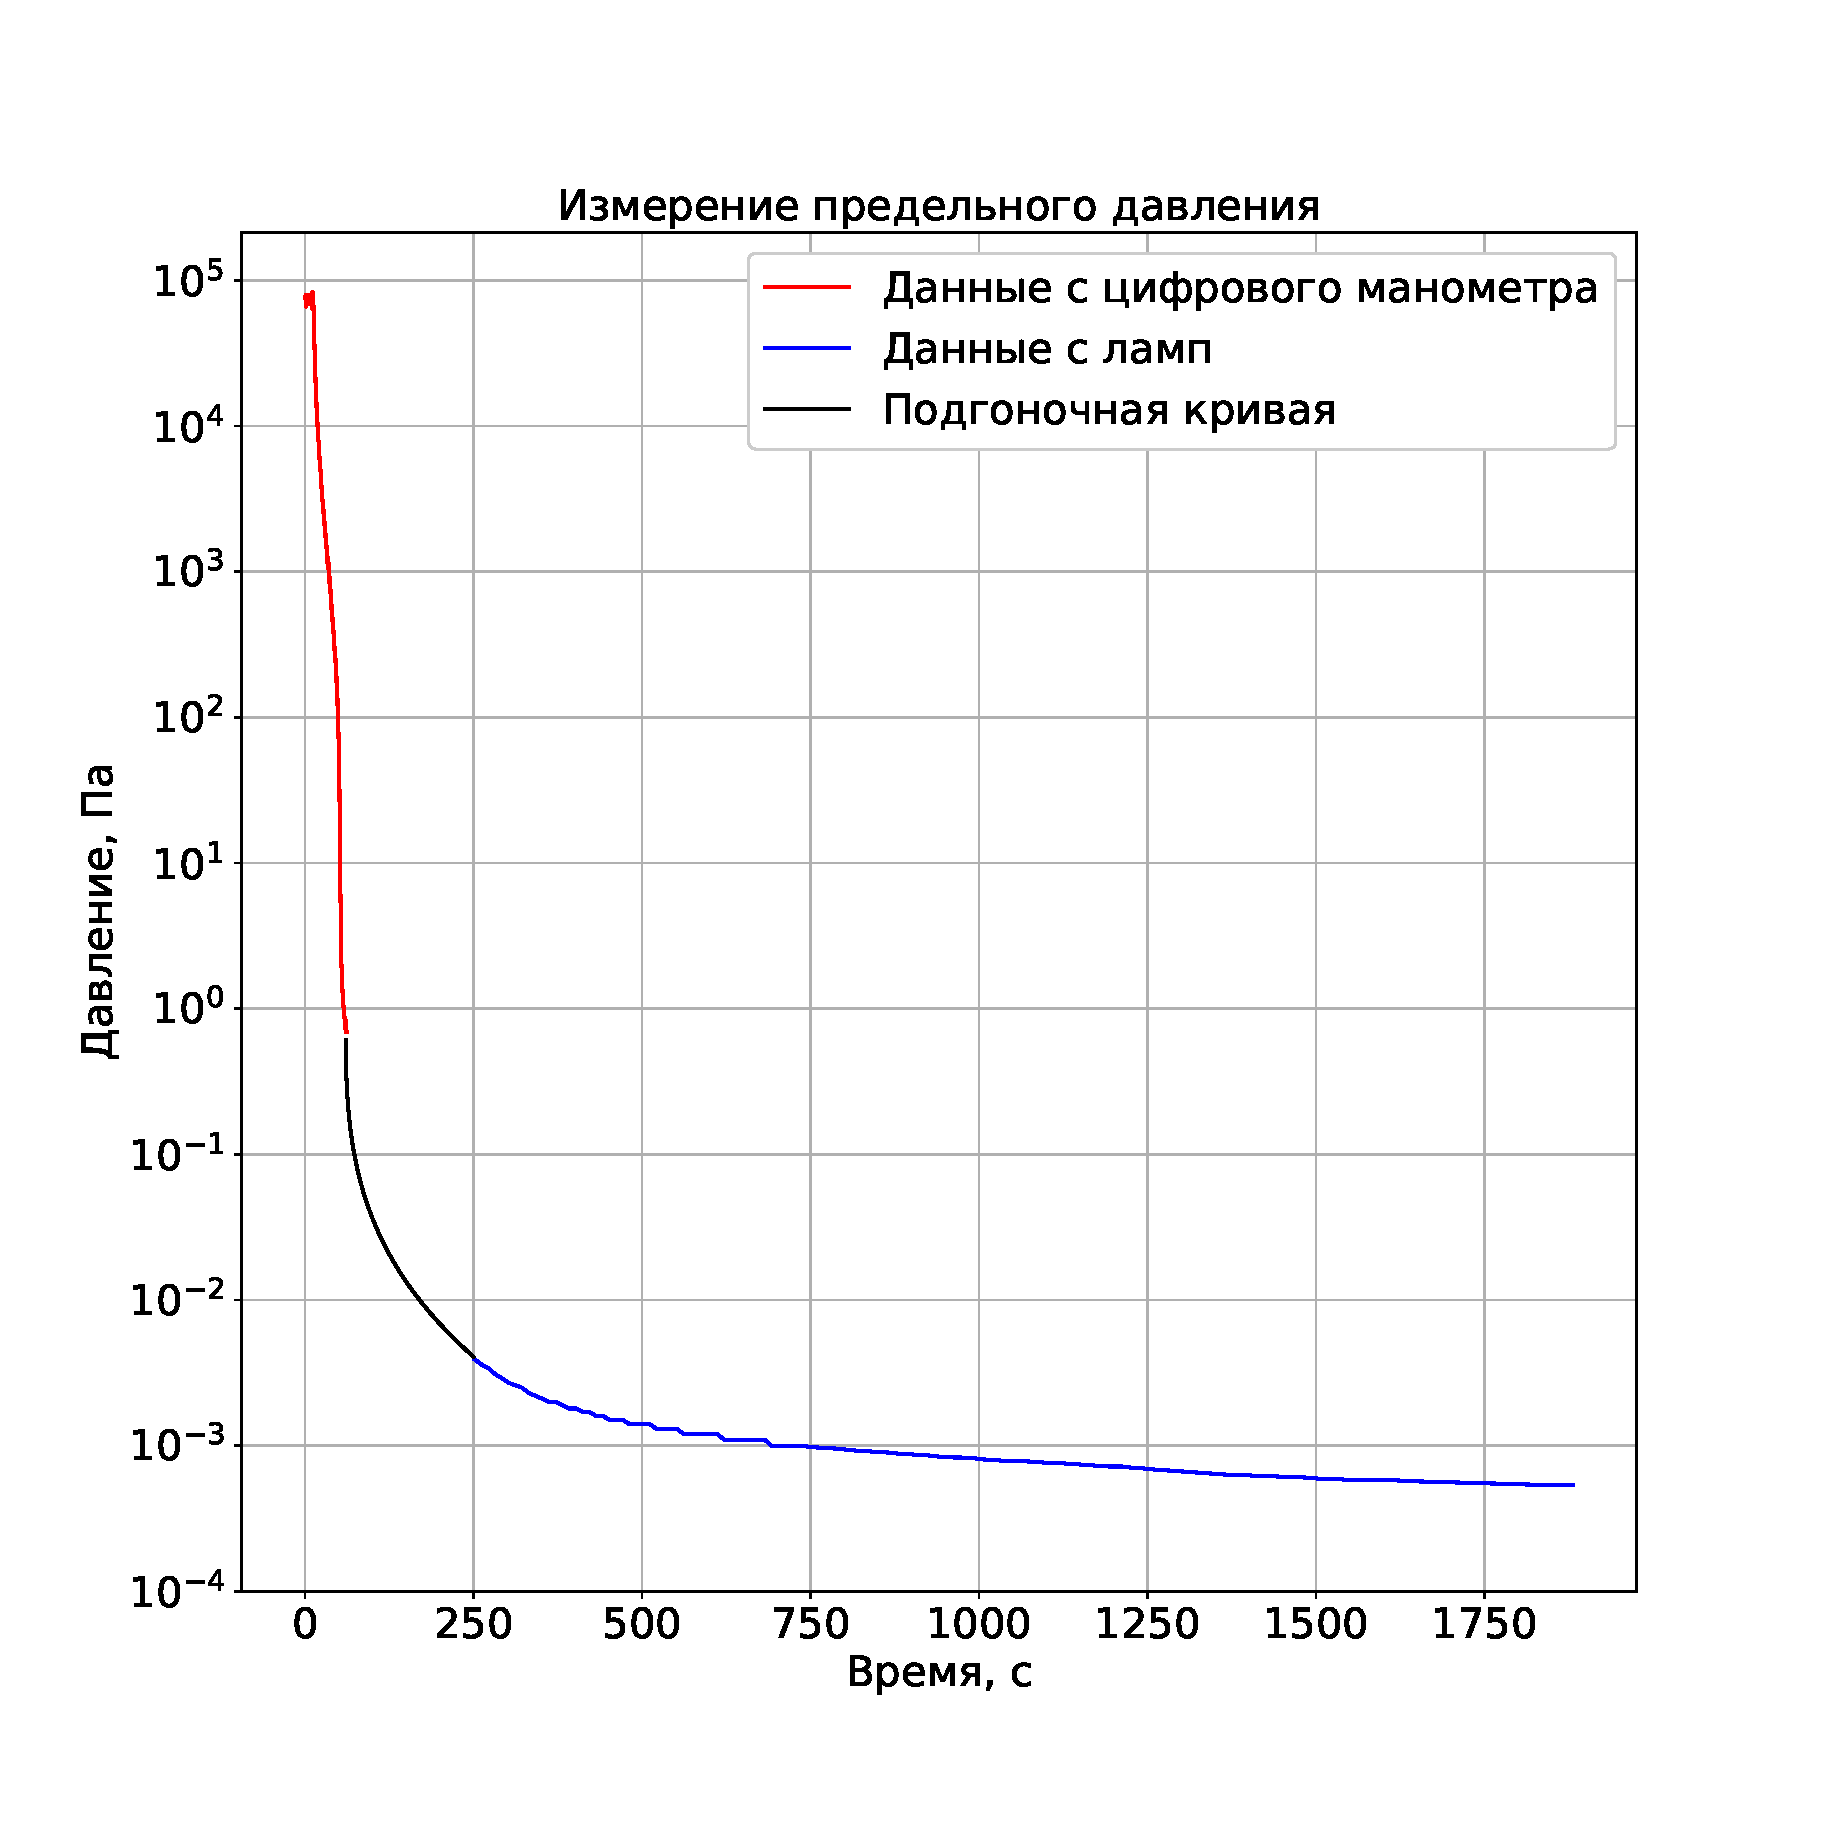
\includegraphics[width=.80\linewidth]{Lab1_1.eps}
					\caption{На графике изображены три прямые: прямая, прямая соответствующая заявленной индуктивности, прямая, построенная по экспериментальным данным с помощью МНК и прямая, построенная с помощью взвешенного МНК}
					\label{fig2}
				\end{figure} 
				\newpage
				С помощью взвешенного МНК была построена прямая, коэффициент которой определяет искомое значение индуктивности катушки \newline $L = 1.1 \pm 0.1 $ мГн
		\subsection{Снятие ВАХ диода}
			\subsubsection{Теория работы}
				Диод – это полупроводниковый прибор с одним p-n переходом, имеющий два	вывода (анод и катод), и предназначенный для выпрямления, детектирования, стабилизации, модуляции, ограничения и преобразования электрических сигналов. Такой прибор может находиться только в одном из двух состояний: 
				\begin{enumerate}
					\item Открытое – когда он хорошо проводит ток.
					\item Закрытое – когда он плохо проводит ток.
				\end{enumerate}
				Зависимость тока, проходящего через p-n переход, от величины и полярности приложенного к нему напряжения изображают в виде кривой, называемой вольтамперной характеристикой (ВАХ) диода.
				\begin{figure}[h]
					\centering
					\includegraphics[width=.40\linewidth]{схема2.png}
					\caption{Схема измерения ВАХ диода. $R$ – резистор, $D$ – диод (прямой и обратный ход), $G$ – выход встроенного генератора осциллографа, $U_x$ и $U_y$ – напряжения, измеряемое на первом и втором каналах осциллографа. Земля у генератора и обоих входов осциллографа общая. С генератора подается синусоидальный сигнал с амплитудой 12 В. Измерения удобно проводить в режиме $XY$. Подача переменного напряжения позволяет снять ВАХ одновременно в положительном и отрицательном направлении.}
					\label{fig3}
				\end{figure}
			\subsubsection{Ход работы}
				В ходе работы с помощью осциллографа на заданной схеме были измерены переменные напряжения $U_x$ и $U_y$, а затем построена ВАХ.
					\begin{figure}[h]
						\centering
						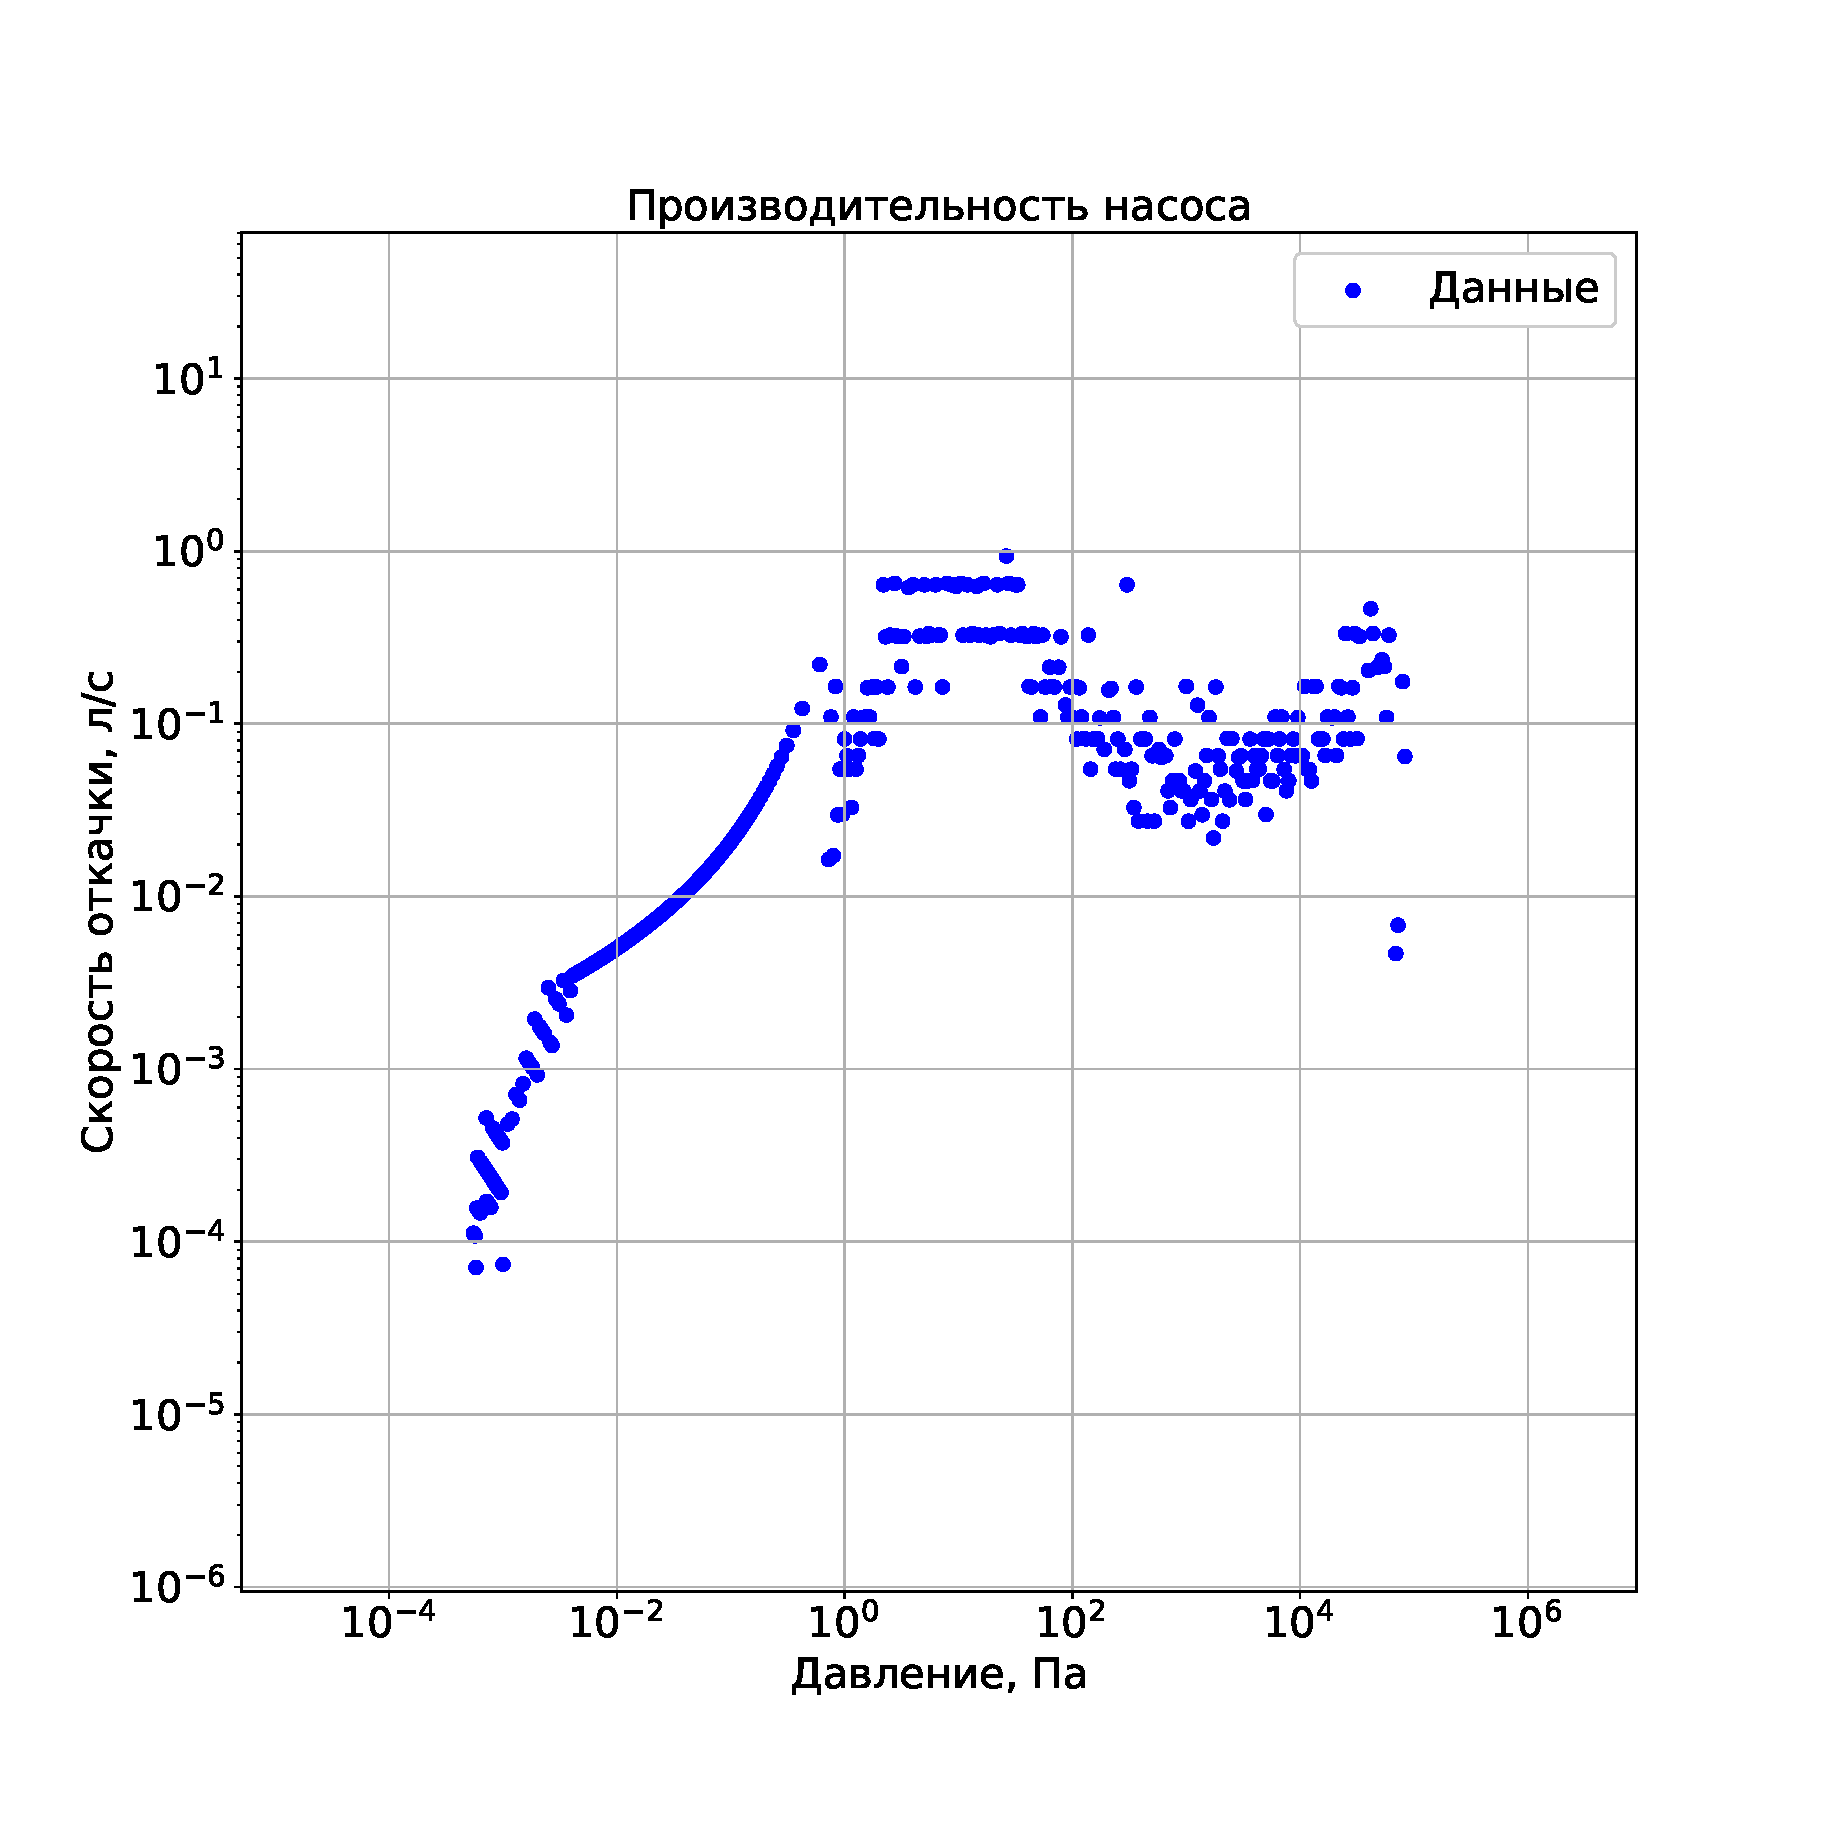
\includegraphics[width=.80\linewidth]{Lab1_2.eps}
						\caption{ВАХ диода}
						\label{fig4}
					\end{figure}
				\newpage
		\subsection{Измерение малого сопротивления}
			\subsubsection{Теория работы}
				Измерить малое сопротивление омметром весьма проблематично, так как так как омметр измерит все сопротивления цепи, включая сопротивления соединительных проводов $R_{wire}$ и сопротивление самого компонента $R_{component}$. Чтобы этого избежать можно использовать 4 проводную схему измерения сопротивления, когда ток и напряжение измеряются независимо друг от друга.
				\begin{figure}[h!]
					\centering
					\includegraphics[width=.40\linewidth]{Схема3.png}
					\caption{4 проводная схема измерения малого сопротивления}
					\label{fig5}
				\end{figure}
				\newpage
				При этом по проводам подключения вольтметра будет идти очень
				незначительный ток, а, следовательно, падение напряжения на них будет таким
				маленьким, что его можно не принимать во внимание. В качестве вольтметра в
				данной работе используется мультиметр, ток задается на источнике постоянного
				тока. Требуется определить сопротивление металлического образца по
				зависимости напряжения на нем от тока. Оценить погрешность измерений.
			\subsubsection{Ход работы}
				В ходе работы с помощью мультиметра и блока питания с амперметром были измерены показания напряжения на образце в зависимости от заданной силы тока на блоке питания.
				\begin{figure}[h]
					\centering
					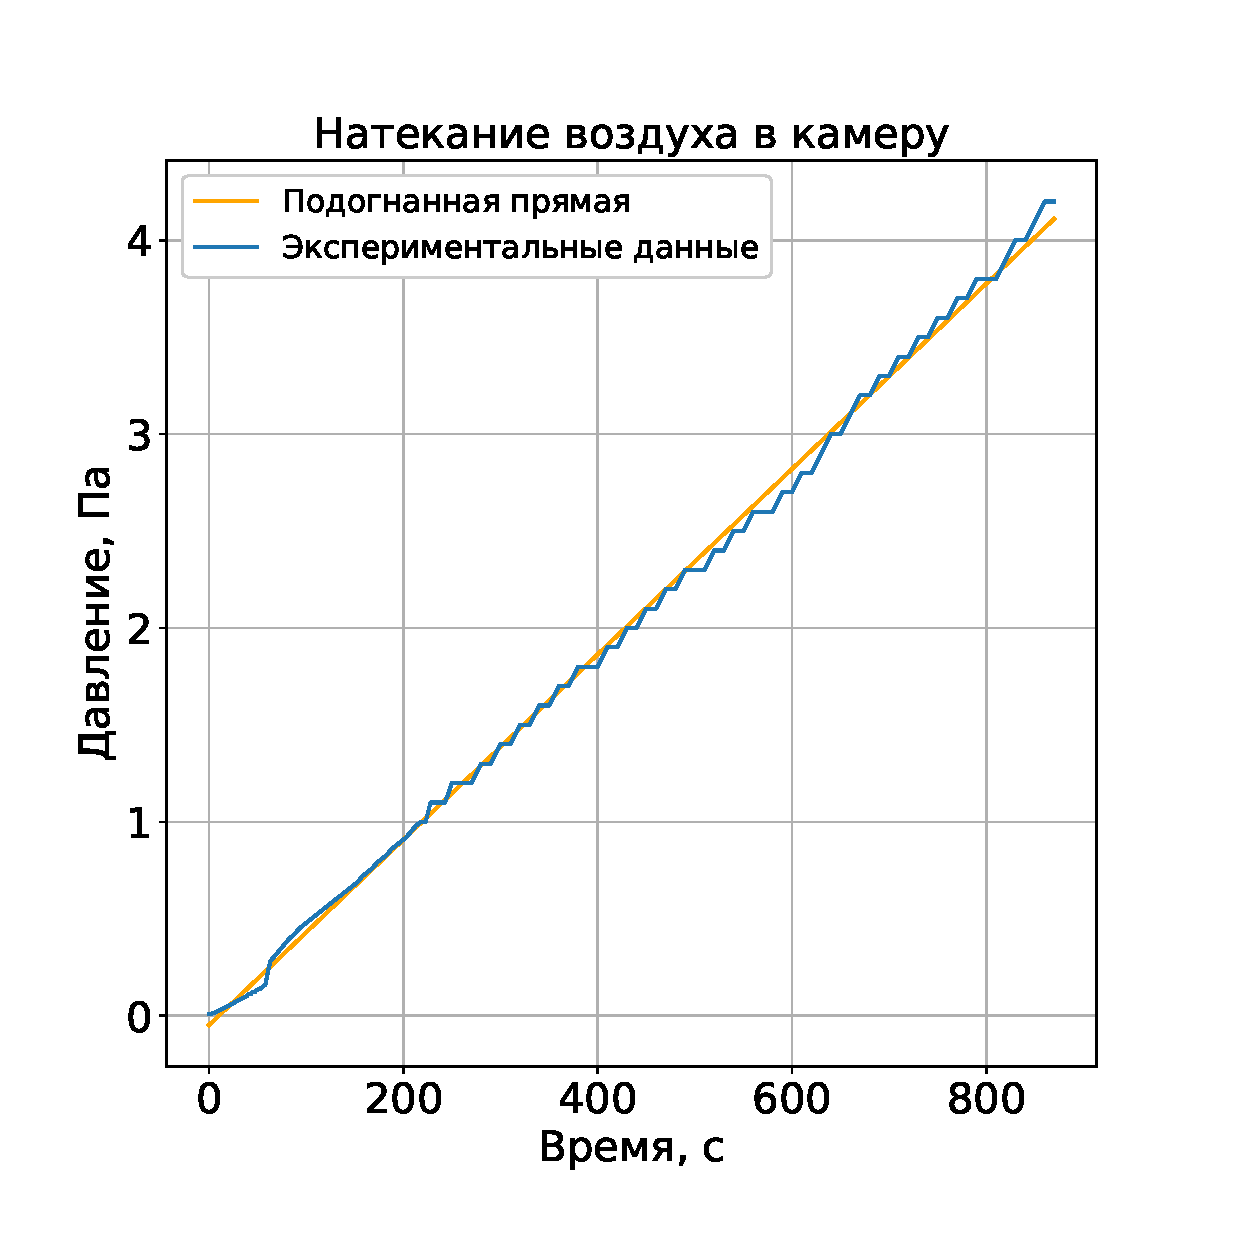
\includegraphics[width=.80\linewidth]{Lab1_3.eps}
					\caption{Зависимость напряжения от тока на образце}
					\label{fig6}
				\end{figure}
				\newpage
				С помощью была МНК построена прямая, коэффициент которой определяет искомое значение сопротивления образца $R = 4.1 \pm 0.1$ мОм
				Различные сплавы латуни могут обладать различными удельными сопротивлениями (отличие до 4 раз), что усложняет теоретический подсчет сопротивления образца.
	\section{Генератор Ван Дер Граафа}
		\subsection{Оборудование}
			\begin{itemize}
				\item Генератор Ван де Граафа 
				\item Источник постоянного тока для питания
				электродвигателя 
				\item Осциллограф 
				\item Щуп для осциллографа – 1 шт. 
				\item Мультиметр 
				\item Высоковольтный кабель для подключения к сфере генератора 
				\item Провода для заземления
			\end{itemize}
		\subsection{Задачи}
			\begin{itemize}
				\item Определить напряжение пробоя воздуха  
				\item Определить напряжение генератора Ван Дер Граафа по длине газового разряда в воздухе
			\end{itemize}
		\subsection{Измерение тока генератора}	
			\subsubsection{Теория работы}
				Измерить ток генератора $I$. Для этого подключить к генератору мультиметр. Напряжение на генераторе задается источником питания. Провести измерения при различных скоростях вращения ленты (задается установкой напряжения на источнике питания).
				\begin{figure}[h]
					\centering
					\includegraphics[width=.30\linewidth]{Схема4.png}
					\caption{Схема измерения тока генератора}
					\label{fig7}
				\end{figure}
				\newpage
			\subsubsection{Ход работы}
				В ходе работы к генератору был подключен мультиметр, ток был измерен при разных напряжениях, подаваемых генератором.
				\begin{figure}[h]
					\centering
					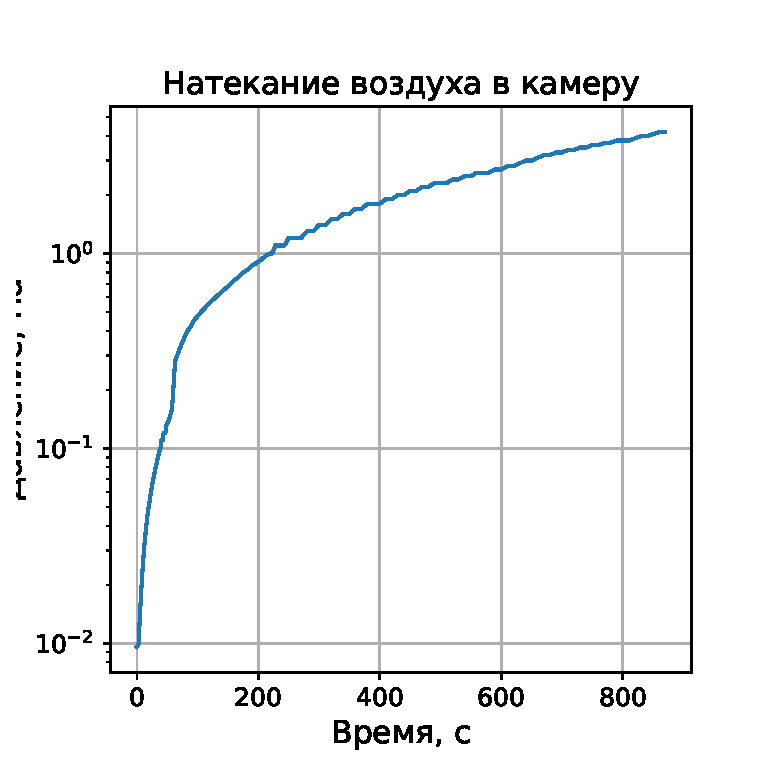
\includegraphics[width=.80\linewidth]{Lab1_4.eps}
					\caption{Зависимость напряжения от тока на генераторе}
					\label{fig8}
				\end{figure}
				\newpage
				С помощью МНК была построена прямая, определяющая коэффициент пропорциональности (сопротивление): $U = 1.132 I + 2.393$
		\subsection{Определение напряжения пробоя воздуха}
			\subsubsection{Теория работы}
				Вернуть обратно малую заземленную сферу. Измерить период искрового разряда $T$ при помощи осциллографа. Для измерения достаточно расположить осциллограф	недалеко от генератора, период наводок на экране осциллографа совпадает с периодами искрового разряда. Следует избегать прямого подключения любых измерительных приборов к высоковольтному генератору. 
				\newline
				Пренебрегая ёмкостью малой сферы, оценить ёмкость большой сферы генератора как $C = 4 \pi \epsilon_0 r$ где $r$ – радиус сферы. 
				\newline
				Измерить период искрового разряда $T$ для различных расстояний между сферами.
				\newline 
				Полученные выше измерения позволяют оценить напряжение пробоя в зависимости от расстояния $d$ между сферами:
				$E_{bd} = \frac{IT}{dC}$
				\newline
				Оценить погрешность измерений.
			\subsubsection{Ход работы}
				В ходе работы были измерены периоды искрового разряда $T$ для разных расстояний при 2 сериях напряжений.
				\begin{figure}[h]
					\centering
				 	\includegraphics[width=.80\linewidth]{Lab1_5.eps}
				 	\caption{Зависимость напряжения от тока на генераторе}
				 	\label{fig9}
				\end{figure}
				\newpage
				С помощью МНК была построена прямая, коэффициентом которой является напряженность пробоя воздуха $E_{bd} = 23 \pm 3$ кВ/см
		\subsection{Оценка напряжений генератора}
			\subsubsection{Теория работы}
				Один из способов измерения больших напряжений – шаровые измерительные разрядники. Порядок измерений высоковольтных напряжений регламентируются в ГОСТ 17512-82 [1]. Напряжение пробоя газов сильно зависит от давления, состава газа и формы
				электродов. Пренебрегая тем, что сферы имеют различный диаметр, определить напряжение генератора для различных скоростей вращения ленты. Для различных расстояний между сферами $d$ определить напряжение по Таблице 1. Для условий отличающихся от нормальных следует использовать поправочный
				коэффициент $k: U_{tr} = k U_{tab}$, где $U_{tab}$– значение разрядного напряжения определенное из Таблицы 1, $U_tr$ - истинное значение напряжения. Для значений относительной плотности воздуха от 0.95 до 1.05 поправочный коэффициент $k$ можно оценить как: $k = 0.386 \frac{P}{273+t}$где давление $P$ выражено в миллиметрах ртутного столба, а температура $t$ в градусах Цельсия.
				\newline
				Сравнить полученные результаты с результатами из первой части работы.
			\subsubsection{Ход работы}
				В ходе работы на графике из предыдущей части была построена зависимость напряжения от расстояния предлагаемая Таблицой 1
				\begin{figure}[h!]
					\centering
					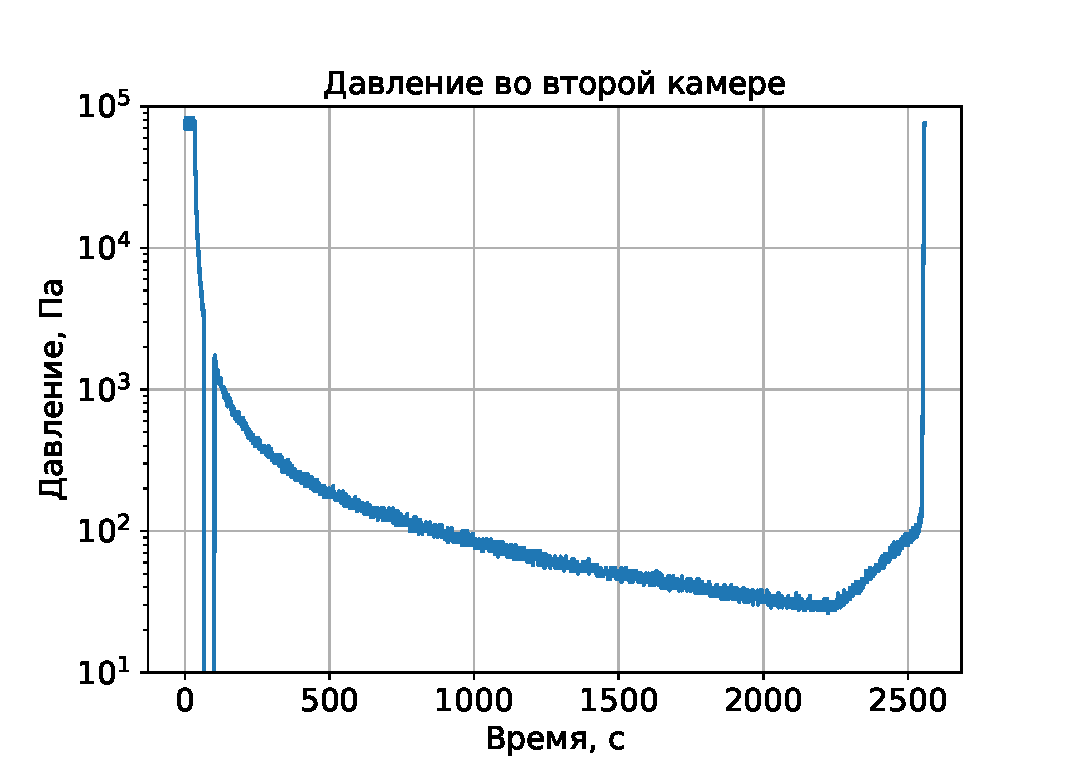
\includegraphics[width=.80\linewidth]{Lab1_6.eps}
					\caption{Зависимость напряжения пробоя воздуха от расстояния между сферами}
					\label{fig10}
				\end{figure}
				\newline
				На график добавилась прямая черного цвета, она соответствует зависимости, построенной по данным из Таблицы 1. Ее коэффициент наклона равен напряженности пробоя воздуха $E_{bd} = 26$ Кв/м. Как можно заметить, коэффициены прямых отличаются, но в пределах погрешности экспериментальных данных.
\end{document}